\documentclass{article}
\usepackage{graphicx}
\usepackage{enumitem}
\usepackage{booktabs}
\usepackage[textwidth=18cm, textheight=26cm]{geometry}

%\setlength{\oddsidemargin}{11pt}% the default is 31pt so decrease by 20pt
%\setlength{\textwidth}{430pt}% the default is 390pt so increase by 40pt

\newcommand{\imgSize}{0.40\textwidth}

\begin{document}
    \pagenumbering{gobble}

    \centerline{\Large{Examples for Markers in Images}}
    \begin{table}[h!]
        \begin{center}
        \begin{tabular}{ c c }
        Input & Segmentation \\ 
        \raisebox{-\totalheight}{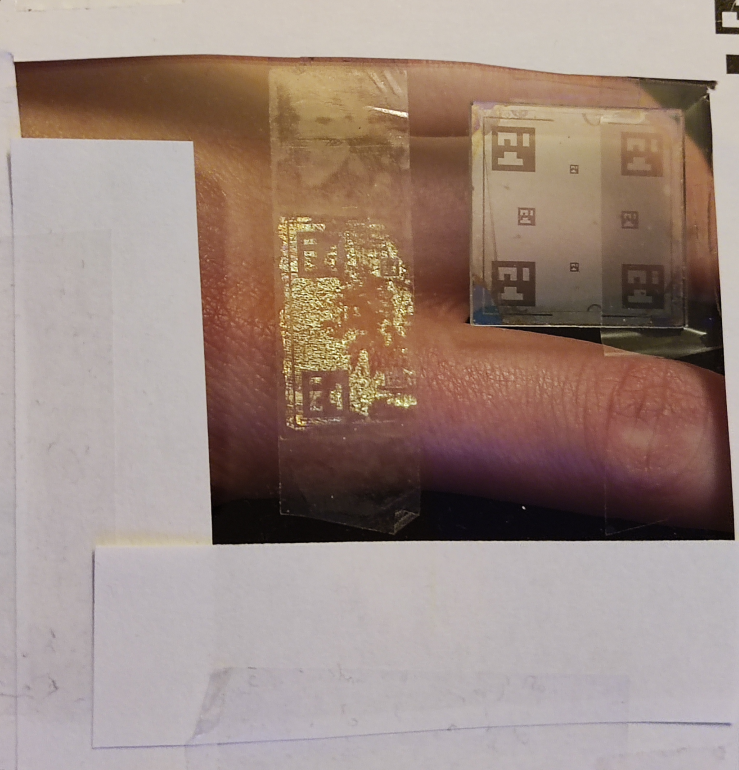
\includegraphics[width=\imgSize, height=\imgSize]{images/75_in.png}} & 
        \raisebox{-\totalheight}{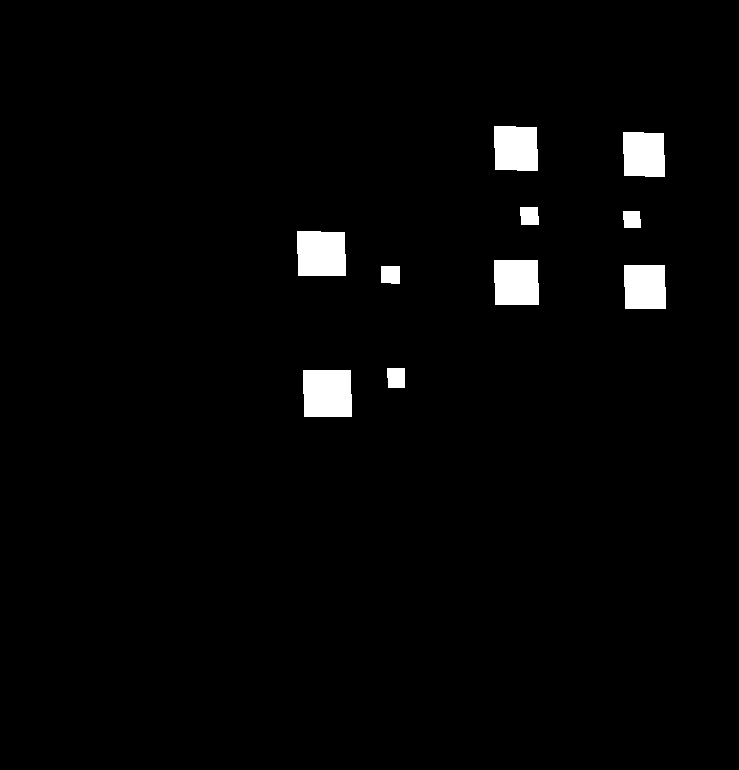
\includegraphics[width=\imgSize, height=\imgSize]{images/75_seg.png}} \\ 
        \raisebox{-\totalheight}{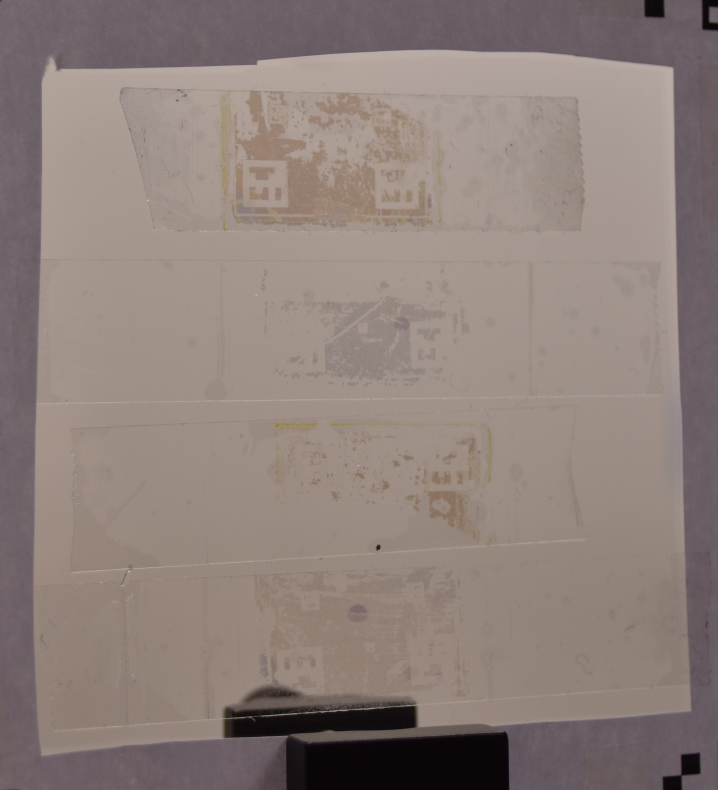
\includegraphics[width=\imgSize, height=\imgSize]{images/107_in.png}} & 
        \raisebox{-\totalheight}{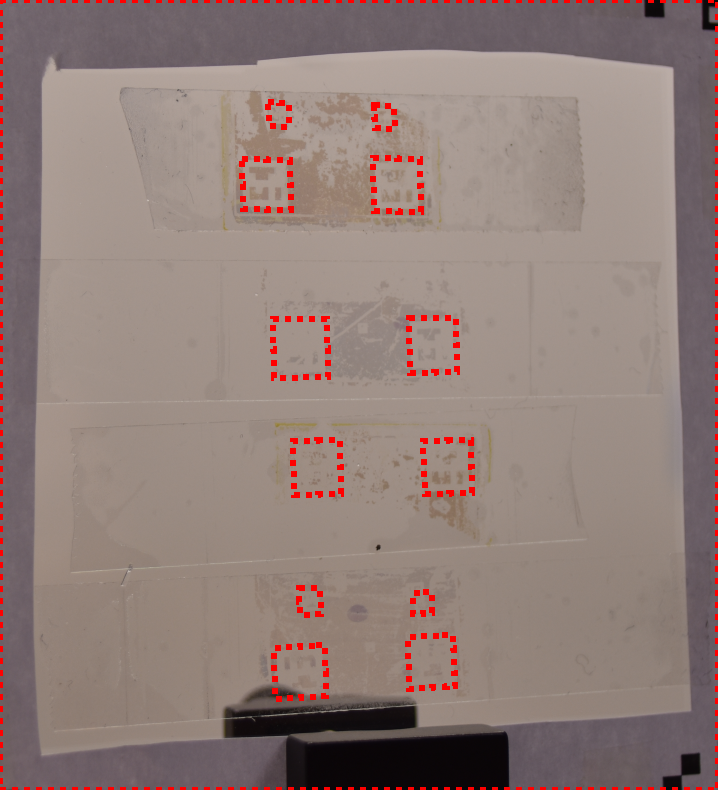
\includegraphics[width=\imgSize, height=\imgSize]{images/107_seg.png}} \\ 
        \raisebox{-\totalheight}{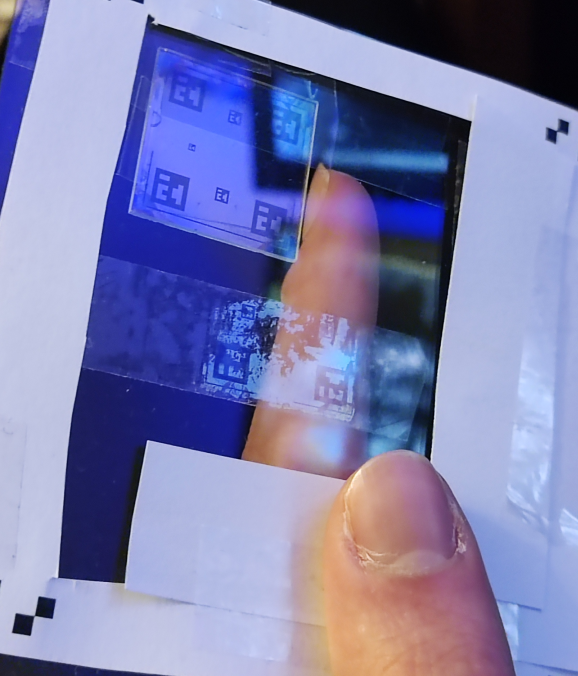
\includegraphics[width=\imgSize, height=\imgSize]{images/112_in.png}} & 
        \raisebox{-\totalheight}{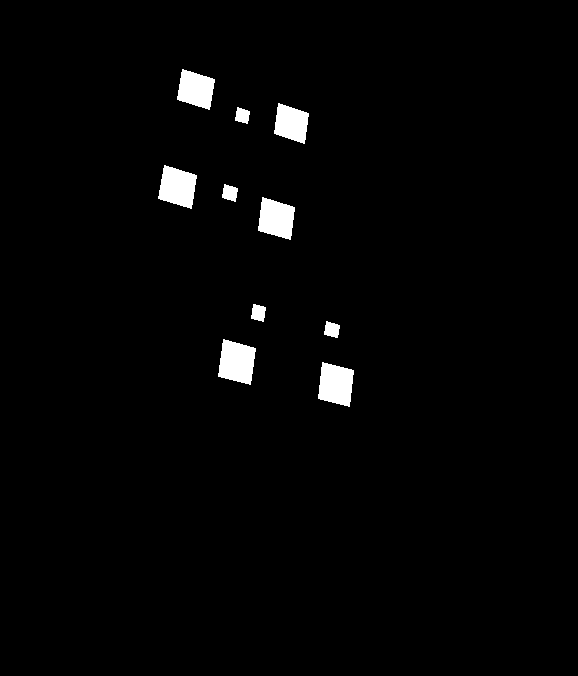
\includegraphics[width=\imgSize, height=\imgSize]{images/112_seg.png}} \\ 
        \end{tabular}
        \label{tbl:pics}
        \end{center}
    \end{table}
\end{document}
